\documentclass{astroedu-lab}

\begin{document}

\pagestyle{plain}

\begin{problem}{\huge Лабораторная работа 2.4.1\\\\Измерение магнитного поля Земли\\\\Выполнил Жданов Елисей Б01-205}

\section{Цель работы:}

1) Определить характеристики шарообразных неодимовых магнитов 

2) Измерить горизонтальную и вертикальную составляющие индукции магнитного поля Земли и магнитное наклонение.

\section{Оборудование:}

12 одинаковых неодимовых магнитных шариков

Тонкая нить для изготовления крутильного маятника

Медная проволока диаметром (0.5 – 0.6) мм

Электронные весы

Секундомер

Измеритель магнитной индукции АТЕ-8702

Штангенциркуль

Брусок из немагнитного материала

Деревянная линейка

Штатив из немагнитного материала

Набор гирь и разновесов

\section{Теоретическая справка}

Простейший магнитный диполь может быть образован витком с током или постоянным магнитом. По определению, магнитный момент $\vec{\mathfrak{m}}$ тонкого витка площадью $S$ с током $I$ равен (в СИ)\[\vec{\mathfrak{m}}=I\vec{S},\]где $\vec{S}=S\vec{n}$ -- вектор площади контура, образующий с направлением тока правовинтовую систему, $\vec{n}$ -- единичный вектор нормали к площадке (это же направление $\vec{\mathfrak{m}}$ принимается за направление $S\to N$ от южного $S$ к северному $N$ полюсу магнита). Если размеры контура с током или магнитной стрелки малы по сравнению с расстоянием до диполя, то соответствующий магнитный диполь $\vec{\mathfrak{m}}$ называют \textit{элементраным} или \textit{точечным}.

Магнитное поле точечного диполя определяется по формуле, аналогичной формуле для поля элементарного электрического диполя:\[\vec{B}_{\text{дип}}=\frac{\mu_0}{4\pi}\left(\frac{3\left(\vec{\mathfrak{m}}\cdot\vec{r}\right)\vec{r}}{r^5}-\frac{\vec{\mathfrak{m}}}{r^3}\right).\]

Во внешнем магнитном поле с индукцией $\vec{B}$ на точечный магнитный диполь $\vec{\mathfrak{m}}$ действует механический момент сил\[\vec{\mathcal{M}}=\left[\vec{\mathfrak{m}}\times\vec{B}\right].\]При этом потенциальная энергия, которой обладает диполь с постоянным $\vec{\mathfrak{m}}$, равна\[W=-\left(\vec{\mathfrak{m}}\cdot\vec{B}\right).\]Когда диполь ориентирован вдоль внешнего поля ($\mathfrak{m}\parallel\vec{B}$), он находится в состоянии \textit{равновесия} ($\vec{\mathcal{M}}=0$). При этом \textit{устойчивым} будет только состояние, в котором диполь \textit{сонаправлен} с полем $\vec{\mathfrak{m}}\uparrow\uparrow\vec{B}$, поскольку его потенциальная энергия достигает \textit{минимума} $(W_{min}=-\mathfrak{m}B)$. При противоположной ориентации энергия будет иметь максимум $W_{max}=\mathfrak{m}B$, и состояние равновесия будет неустойчивым.

В \textit{неоднородном} внешнем поле выражение для энергии постоянного диполя сохраняется. При этом кроме момента сил на диполь действует ещё и сила\[\vec{F}=-\nabla W=\left(\vec{\mathfrak{m}}\cdot\nabla\right)\vec{B}.\]В частности, проекция этой силы на ось $x$ имеет вид\[F_x=\mathfrak{m}_x\frac{\partial B_x}{\partial x}+\mathfrak{m}_y\frac{\partial B_y}{\partial y}+\mathfrak{m}_z\frac{\partial B_z}{\partial z}.\]Таким образом, \textit{свободный} магнитный диполь в неоднородом магнитном поле ориентируется вдоль силовых линий магнитного поля и втягивается в область более сильного поля, поскольку это ведёт к уменьшению энергии диполя.

Рассчитаем силу взаимодействия магнитов с моментами $\vec{\mathfrak{m}}_1$ и $\vec{\mathfrak{m}}_2$ в рамках модели точечных диполей. В частном случае, когда моменты двух небольших магнитов направлены вдоль соединяющей их прямой: $\vec{\mathfrak{m}}_{1,2}\parallel\vec{r}$, где $\vec{r}$ -- радиус-вектор между ними, магниты взаимодействуют с силой\[F_{12}=\mathfrak{m}_1\frac{\partial B_2}{\partial r}=\mathfrak{m}_1\frac{\partial\left(\frac{2\mathfrak{m}_2}{r^3}\right)}{\partial r}=-\frac{6\mathfrak{m}_1\mathfrak{m}_2}{r^4}\ \text{(ед. СГС).}\]Здесь магниты притягиваются, если их магнитные моменты сонаправлены $(\vec{\mathfrak{m}}_1\uparrow\uparrow\vec{\mathfrak{m}}_2)$, и отталкиваются, если направлены противоположно $(\vec{\mathfrak{m}}_1\uparrow\downarrow\vec{\mathfrak{m}}_2)$.

Если магнитные моменты направлены перпендикулярно соединяющей их прямой: $\vec{\mathfrak{m}}_{1,2}\perp\vec{r}$, то нетрудно показать, что сила их взаимодействия окажется в два раза меньшей и будет иметь противоположный знак:\[F_{12}=\frac{3\mathfrak{m}_1\mathfrak{m}_2}{r^4}\ \text{(ед. СГС)}\](диполи притягиваются при $\vec{\mathfrak{m}}_1\uparrow\downarrow\vec{\mathfrak{m}}_2$ и отталкиваются при $\vec{\mathfrak{m}}_1\uparrow\uparrow\vec{\mathfrak{m}}_2$).

Для проведения эксперимента важно, что, во-первых, вещество, из которого изготовлены магниты, является \textit{магнитожёстким} материалом, и, во-вторых, шары намагничены однородно.

"Магнитожёсткость" материала означает, что магнитные моменты шаров в процессе работы не изменяются под действием внешних магнитных полей, т. е. шар ведёт себя как постоянный ("жёсткий") диполь. В том числе, магнитные моменты не изменяются при контакте магнитов друг с другом.

Магнитное поле однородно намагниченного шара радиусом $R$ может быть вычислено точно. На расстояниях $r\geq R$ от центра шара оно совпадает с полем точечного магнитного диполя, расположенного в центре, магнитный момент $\mathfrak{m}$ которого совпадает с полным моментом шара. Внутри шара магнитное поле однородно -- нетрудно получить, что при $r < R$\[\vec{B}_0=\frac{\mu_0\vec{\mathfrak{m}}}{2\pi R^3}\ \left[\text{СИ}\right].\]

В качестве ещё одной характеристики материала магнита используют остаточную \textit{намагниченность} $\vec{M}$. По определению, намагниченность равна \textit{объёмной плотности магнитного момента}, поэтому для однородно намагниченного шара\[\vec{\mathfrak{m}}=\vec{M}V,\]где $V=\frac{4\pi}{3}R^3$ -- объём магнита. Величину $\vec{B}_r=\mu_0\vec{M}$ называют \textit{остаточной индукцией} материала.

Нетрудно видеть, что индукция $\vec{B}_p$ \textit{на полюсах} однородно намагниченного шара неправлена по нормали к поверхности и совпадает поэтому с индукцией внутри шара: $\vec{B}_p=\vec{B}_0$. Тогда величина $B_p$ связана с остаточной индукцией $B_r$ соотношением\[B_p=B_0=\frac{2}{3}B_r.\]

\section{Экспериментальная установка}

\subsection{Определение величины магнитного момента шариков}

Величину магнитного момента $\mathfrak{m}$ одинаковых шариков можно рассчитать, зная их массу $m$ и определив максимальное расстояние $r_{max}$, на котором они ещё удерживают друг друга в поле тяжести. При максимальном расстоянии сила тяжести шариков равна силе их магнитного притяжения:\[\frac{6\mathfrak{m}^2}{r_{max}^4}=mg\implies\mathfrak{m}=\sqrt{\frac{mgr_{max}^4}{6}}.\]

По величине магнитного момента $\mathfrak{m}$ можно рассчитать величину индукции магнитного поля вблизи любой точки на поверхности шара радиуса $R$. Максимальная величина индукции наблюдается на полюсах:\[\vec{B}_p=\frac{2\vec{\mathfrak{m}}}{R^3}.\]

Величину магнитного момента шариков можно определить макже по силе их сцепления. Она определяется как сила, необходимая для разрыва двух сцепившихся магнитных шариков. Сила сцепления максимальна, если шары соединяются своими противоположными полюсами.

Максимальную силу сцепления можно определить по весу магнитной цепочки, которую способен удержать самый верхний магнитный шарик. Если цепь состоит из одинаковых магнитных шариков, то при определённой длине она она оторвётся от верхнего шарика. Приэтом, учитывая, что сила приятжения убывает как $F\sim\frac{1}{r^4}$, для расчёта прочности цепочки достаточно учитывать силу взаимодействия верхенего шара с тремя-четырьмя ближайшими соседями.

Если сила сцепления двух одинаковых шаров диаметром $d$ с магнитными моментами $\mathfrak{m}$ равна\[F_0=\frac{6\mathfrak{m}^2}{d^4},\]то минимальный вес цепочки, при которой она оторвётся от верхнего шарика, равен\[F=F_0\sum_{n=1}^{+\infty}\frac{1}{n^4}=\frac{\pi^4}{90}F_0\approx1,08F_0.\]

Таким образом, сила сцепления двух шаров равна\[F_0=\frac{90}{\pi^4}F=0,924F.\]

\subsection{Измерение горизонтальной составляющей индукции магнитного поля Земли}

Магнитное поле в настоящей работе определяется по периоду крутильных колебаний магнитной стрелки вокруг вертикальной оси.

"Магнитная стрелка" образована из сцепленных друг с другом противоложными полюсами шариков и с помощью $\Lambda$-образного подвеса подвешена в горизонтальном положении. Магнитные моменты шариков направлены в одну сторону вдоль оси "стрелки". Под действием вращательного момента $\vec{M}=\vec{\mathfrak{m}}_0\times\vec{B}$ магнитный момент "стрелки" $\vec{\mathfrak{m}}_0$ выстроится вдоль горизонтальной составляющей магнитного поля Земли $\vec{B}_h$ в направлении $S\to N$. При отклонении "стрелки" на угол $\theta$ от равновесного положения в горизонтальной плоскости возникают крутильные колебания вокруг вертикальной оси, проходящей через середину "стрелки". Если пренебречь упругостью нити, то уравнение крутильных колебаний такого маятника при малых амплитудах ($\sin{\theta}\approx\theta$) имеет вид\[I_n\ddot{\theta}+\mathfrak{m}_0B_h\theta=0,\]где $I_n=\frac{1}{12}m_{\text{ст}}l_{\text{ст}}^2=\frac{1}{12}n^3md^2$ -- момент инерции "стрелки" , состоящей из $n$ шариков, который можно с хорошей точностью приблизить моментом инерции тонкого однородного стержня соответствующей массы и длины, а $\mathfrak{m}_0=n\mathfrak{m}$ -- полный магнитный момент стрелки.

Таким образом, период колебаний маятника оказывается равен\[T(n)=2\pi\sqrt{\frac{md^2}{3\mathfrak{m}B_h}}n=kn,\]где $k=2\pi\sqrt{\frac{md^2}{3\mathfrak{m}B_h}}$.

\subsection{Измерение вертикальной составляющей индукции магнитного поля Земли. Магнитное наклонение.}

Для измерения вертикальной составляющей $B_v$ вектора индукции поля Земли используется та же установка, что и для измерения горизонтальной составляющей с тем лишь отличием, что магнитная "стрелка" подвешивается на нити без $\Lambda$-образного подвеса. В этом случае магнитная "стрелка" , составленная из чётного числа шариков и подвешенная на тонкой нити за середину, расположится не горизонтально, а под некоторым отличным от нуля углом к горизонту. Это связано с тем, что вектор $\vec{B}$ индукции магнитного поля Земли в общем случае не горизонтален, а образует с горизонтом угол $\beta$, зависящий от географической широты $\varphi$ места, где проводится опыт. Величина угла $\beta$ называется магнитным наклонением.

С помощью небольшого дополнительного грузика "стрелку" можно "выровнять" , расположив её горизонтально. В этом случае момент силы тяжести груза относительно точки подвеса будет равен моменту сил, действующих на "стрелку" со стороны магнитного поля. Если масса уравновешивающего груза равна $m_{\text{гр}}$, плечо силы тяжести $r_{\text{гр}}$, а полный магнитный момент "стрелки" $\mathfrak{m}_0=n\mathfrak{m}$, то в равновесии\[m_{\text{гр}}gr_{\text{гр}}=n\mathfrak{m}B_v,\]где $B_v$ -- вертикальная составляющая поля Земли. Видно, что момент $M(n)$ силы тяжести уравновешивающего груза пропорционален числу $n$ шариков, образующих магнитную "стрелку" :\[M(n)=An,\]где $A=\mathfrak{m}B_v$.

\section{Измерения, Обработка}

\subsection{Задание №1 Определение магнитного момента, намагниченности и остаточной магнитной индукции вещества магнитных шариков}

\subsubsection{Метод А}

\begin{figure}[!h]
	\centering
	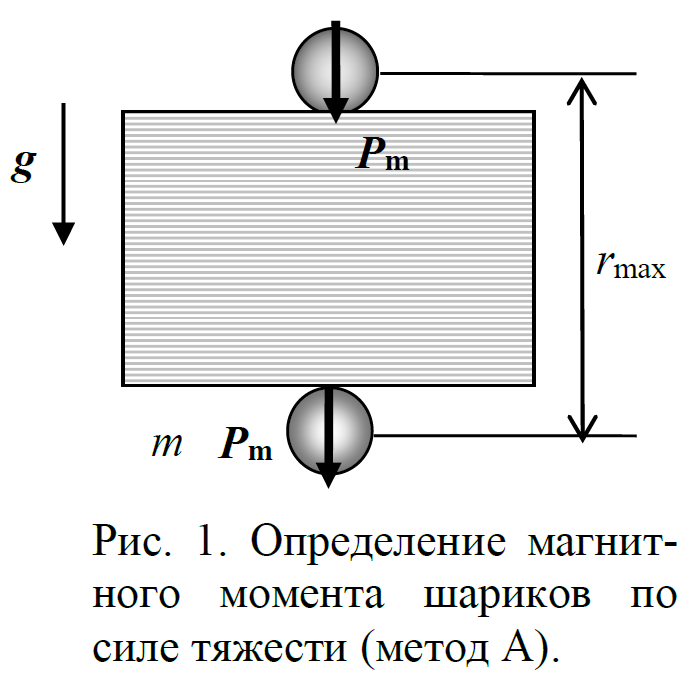
\includegraphics[width=0.4\textwidth]{1.png}
	\label{fig:boiler}
\end{figure}

1) Масса 10 шаров $10m = 8.349$ г. Соответственно, одного шара

\begin{equation}
	m = 0.8349 \text{ г}
\end{equation}

Диаметр шаров замеряем микрометром

\begin{equation}
	D = 0.600 \pm 0.001 \text{ см}
\end{equation}

2) Убедившить, что расстояние замерено при плотно прижатых листах бумаги к фанере, запишем его

\begin{equation}
	r_{max} = 1.66 \pm 0.03 \text{ см}
\end{equation}

3) Тогда магнитный момент

\begin{equation}
	P_m = \sqrt{\frac{m g r_{max}^4}{6}} = 32.4 \pm 1.2 \text{ СГСЭ}
\end{equation}

4) Намагниченность шаров

\begin{equation}
	p_m = \frac{P_m}{\frac{4}{3} \pi R^3} = 285 \pm 11 \text{ Гс}
\end{equation}

5) Величина магнитного поля на полюсах шара

\begin{equation}
	B_p = \frac{2 P_m}{R^3} = 2390 \pm 90 \text{ Гс} = 0.239 \pm 0.009 \text{ Тс}
\end{equation}

Показания магнетометра же

\begin{equation}
	B_p \approx 0.300 \text{ Тс}
\end{equation}

Результаты совпадают более чем хорошо, с учетом того, что показания магнетометра очень чувствительны к положению шарика

6) Остаточная намагниченность

\begin{equation}
	B_r = 4 \pi p_m = 3580 \pm 140 \text{ Гс} = 0.358 \pm 0.014 \text{ Тс}
\end{equation}

Табличное же значение

\begin{equation}
	B_r \approx 1.2 \text{ Тс}
\end{equation}

что позволяет с полной уверенностью заявить о том, что магниты поддельные, и состоят из центрального неодимового сердечника и толстого внешнего гальванического никелевого покрытия.

\subsubsection{Метод Б}

\begin{figure}[!h]
	\centering
	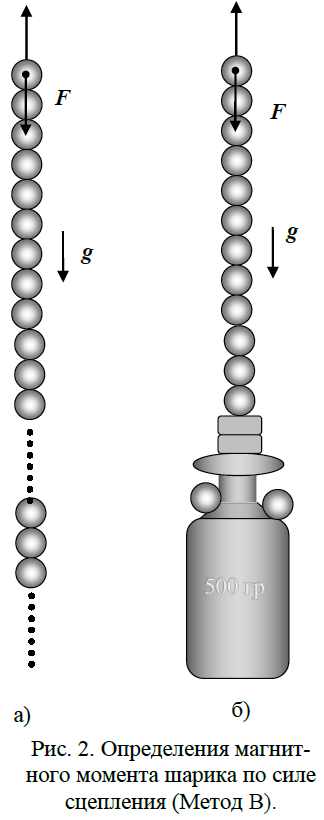
\includegraphics[width=0.37\textwidth]{2.png}
	\label{fig:boiler}
\end{figure}

7) Масса цепочки в момент отрыва

\begin{equation}
	M = 242.3 \pm 0.8 \text{ г}
\end{equation}

8) Вес цепочки

\begin{equation}
	F = M g = 237800 \pm 800 \text{ Дн}
\end{equation}

9) Сила сцепления 2-х шариков(коэффициент в пределе заменен на дзета-функцию Римана $\zeta(4)$)

\begin{equation}
	F_0 = \frac{90}{\pi^4} \cdot F = 219700 \pm 700 \text{ Дн}
\end{equation}

10) Магнитный момент шарика

\begin{equation}
	P_m = \sqrt{\frac{F \cdot D^4}{6}} = 68.9 \pm 0.11 \text{ СГСЭ}
\end{equation}

11) Величина поля на полюсах шара

\begin{equation}
	B_p = \frac{2 P_m}{R^3} = 5103 \pm 8 \text{ Гс} = 0.5103 \pm 0.0008 \text{ Тс}
\end{equation}

Значения уже довольно существенно отличаются от показаний магнетометра

12-13) Говорить о точности измерений в данном эксперименте более не приходится, поскольку она - следствие некорректности модели. Значения из метода А соответствуют показаниям магнетометра, при этом они существенно дальше от действительности, нежели значения из метода Б, который дает большее значение магнитного поля за счет усреднения по квазибесконечной цепочки шаров. Тем не менее, как лабораторную характеристику шара, предпочтительнее взять измерение из пункта А.

\begin{equation}
	\boxed{P_m = 32.4 \pm 1.2 \text{ СГСЭ}}
\end{equation}

\newpage

\subsection{Задание № 2 Определение горизонтальной составляющей магнитного поля Земли}

\begin{figure}[!h]
	\centering
	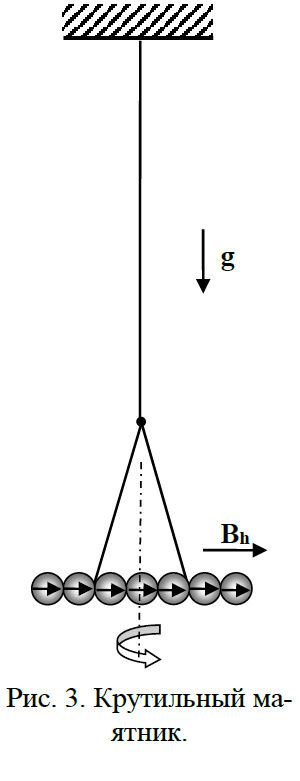
\includegraphics[width=0.28\textwidth]{3.png}
	\label{fig:boiler}
\end{figure}

14-16) Соберем установку и занесем результаты в таблицу

Для значений n от 3 до 7 количество колебаний для расчета периода было взято за 20, далее за 10. В таблицу данные пересчитаны под 1 колебание.

\begin{center}
\begin{tabular}{|c|c|}
\hline 
n, ед & $\tau$, сек \\
\hline
3 & 1.391 \\
4 & 2.002 \\
5 & 2.331 \\
6 & 2.776 \\
7 & 3.248 \\
\hline
8 & 3.677 \\
9 & 4.204 \\
10& 4.628 \\
11& 5.099 \\
12& 5.547 \\
\hline
\end{tabular}
\end{center}

\newpage

\begin{figure}[!h]
	\centering
	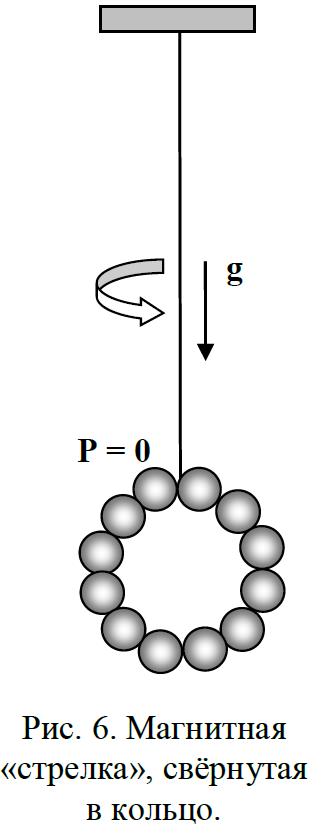
\includegraphics[width=0.25\textwidth]{5.png}
	\label{fig:boiler}
\end{figure}

Для немагнитного кольца период колебаний получился ориентировочно 20 секунд, что действительно свидетельствует о пренебрежимой малости коэффициента упругости нити, к тому же с учетом того, что измерения проводились на порядка 50 проворотах отнисительно положения равновесия маятника, что позволяет им пренебречь.

\newpage

17) График

\begin{center}
	\Large $T(n)$
\end{center}

\begin{figure}[!h]
	\centering
	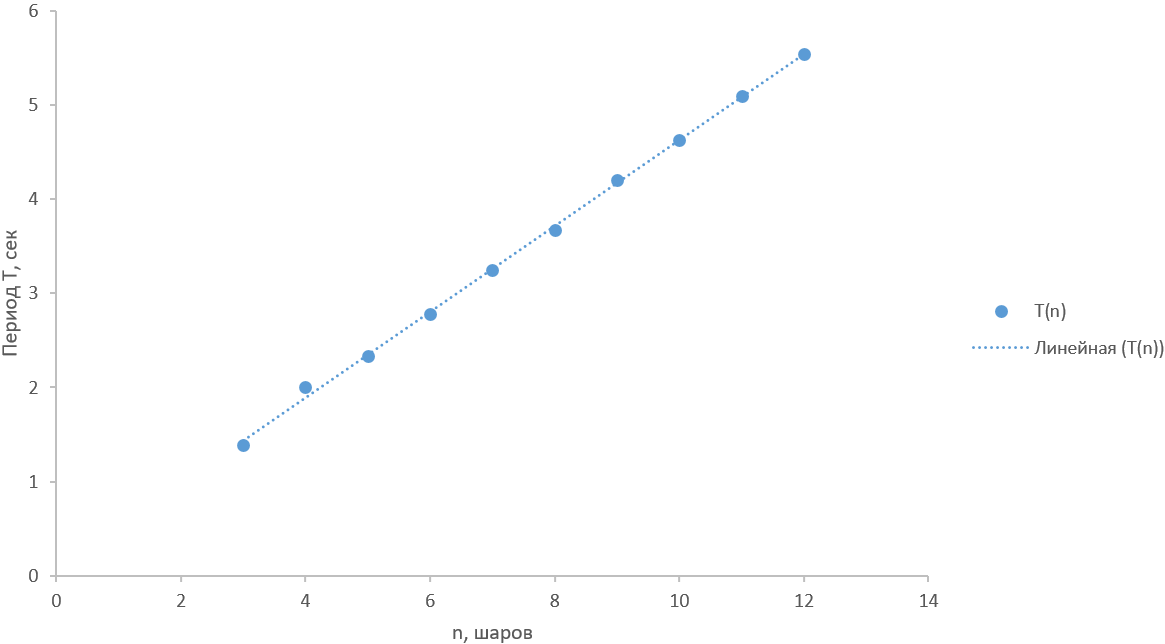
\includegraphics[width=1\textwidth]{график1.png}
	\label{fig:boiler}
\end{figure}

18) Найдем угловые коэффициенты прямой для установки по МНК.

\[
	a = \frac{<x_i y_i> - < x > < y_i >}{< x_i^2> - < x_i >^2}
\]

\[
	b = < \nu_i > - a < N_i >
\]

Также рассчитаем их погрешности

\begin{equation}
	S_a^2 = \frac{< x_i^2>}{< x_i^2 > - < x_i >^2} \cdot \frac{<  b_i - b > ^2}{n - 2}
\end{equation}

Получим прямую

\begin{equation}
	y = (0.4562 \pm 0.0052) \cdot x
\end{equation}

19) Величина горизонтальной составляющей магнитного поля Земли

\begin{equation}
	B_h = \frac{\pi ^ 2 m D^2 }{3 k^2 P_m} = 0.147 \pm 0.009 \text{ Гс}
\end{equation}

Значение получилось близким к табличному

\subsection{Задание № 3 Определение вертикальной составляю-щей магнитного поля Земли}

\begin{figure}[!h]
	\centering
	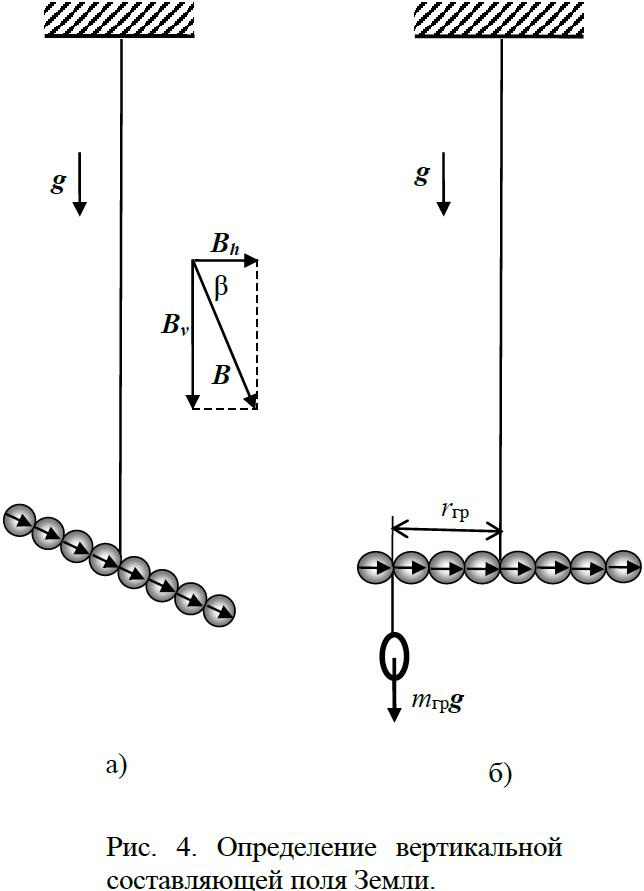
\includegraphics[width=0.6\textwidth]{4.png}
	\label{fig:boiler}
\end{figure}

20-23) Составим таблицу из измеренных и пересчитанных значений

\begin{center}
\begin{tabular}{|c|c|c|c|}
\hline 
n, ед & $n_\text{плечо}$, ед & $m_\text{г}$, грамм & $M$, дин $\cdot$ см \\
\hline
4  & 1 & 0.312 & 184 \\
6  & 2 & 0.253 & 298 \\
8  & 3 & 0.256 & 452 \\
10 & 4 & 0.272 & 641 \\
12 & 5 & 0.212 & 624 \\
\hline
\end{tabular}
\end{center}

\newpage

24) График зависимости

\begin{center}
	\Large $M(n)$
\end{center}

\begin{figure}[!h]
	\centering
	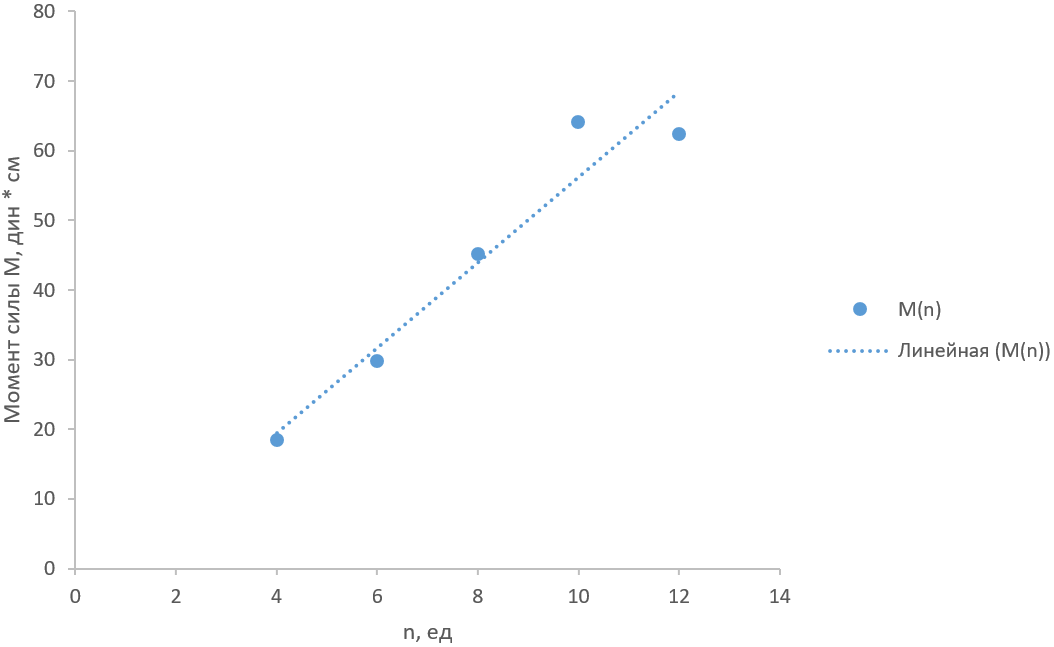
\includegraphics[width=1\textwidth]{график2.png}
	\label{fig:boiler}
\end{figure}

25) По МНК уравнение прямой

\begin{equation}
	y = (6.12 \pm 0.94) \cdot x
\end{equation}

26) Величина вертикальной составляющей магнитного поля Земли

\begin{equation}
	B_\nu = \frac{A}{P_m} = 0.19 \pm 0.03 \text{ Гс}
\end{equation}

27) Магнитное наклонение

\begin{equation}
	\beta = arctg\left(\frac{B_h}{B_\nu}\right) = 52^\circ \pm 7^\circ
\end{equation}

Индукция магнитного поля Земли

\begin{equation}
	B = \sqrt{B_h^2 + B_\nu^2} = 0.24 \pm 0.03 \text{ Гс}
\end{equation}

Полный магнитный момент Земли

\begin{equation}
	P_\oplus = \frac{B R_\oplus^3}{\sqrt{3 sin^2(\varphi) + 1}} = (4.0 \pm 0.4) \cdot 10^{25} \text{ СГСЭ}
\end{equation}

\section{Вывод}

Полученные значение $B = 0.24 \text{ Гс}$ и $\beta = 52^\circ$ довольно близки к табличным величинам $B = 0.065 \text{ Гс}$ и $\beta =72^\circ$. Полученное различие может быть обусловнено массой факторов, начиная от обнаруженного вначале отличия остатой намагниченности шаров до магнитных наводок в основном из-за присутствия в стенах лаборатории стальной арматуры и прочих установок(токамак). 

\section{Ресурсы}

Расчет по МНК: метод-наименьших-квадратов.рф

\end{problem}
\end{document}